% !TEX root = main.tex
\section{System Design and Implementation}
The new conditions of optimality presented above for the \sysIJ\ and \sysIJN\ systems introduce some new design challenges. In the subsequent sections we will detail the design problems that were faced along the way towards implementation and how they were addressed.

During this project, we began by writing a C program implement the \sysII\ system, and then adapted it for the \sysIIN\ system by modifying the conditions of optimality as was outlined in the previous section. We then wrote a C program of the \sysIJ\ system without channel noise. To interface with images, we wrote a Python wrapper program. GNU Octave, MathWorks MATLAB, and Python were used to produce data and create plots.

\subsection{Conditions of Optimality}
We begin by writing out the nearest neighbor conditions for the \sysIJN\ system. To begin, the expressions for $d_X^N(x,i)$ and $d_Y^N(y,j)$ are expanded as follows:
\begin{align}
    \label{eq:int_dist_x}
    d_X^N(x,i)=&E[Y^2 | X = x] +\\
    &\sum_{j=1}^{N_Y} \sum_{k=1}^{N_X} \sum_{l=1}^{N_Y} ( {(x-x_{k,l})}^2 -
    2y_{k,l}E[Y|X=x,Y\in R_j^Y] + y_{k,l}^2 )P(Y\in R_j^Y|X=x)
    P(k,l|i,j)\nonumber\\
    \label{eq:int_dist_y}
        d_Y^N(y,j)=&E[X^2 | Y = y] +\\
    &\sum_{i=1}^{N_X} \sum_{k=1}^{N_X} \sum_{l=1}^{N_Y} ( {(y-y_{k,l})}^2 -
    2x_{k,l}E[X|Y=y,X\in R_i^X] + x_{k,l}^2 )P(X\in R_i^X|Y=y)
    P(k,l|i,j)\nonumber
\end{align}

It is important to note how the nearest neighbor condition for $X$ depends on the $Y$ encoding, and vice versa. It was therefore necessary to adapt the Lloyd-Max iteration because this means the two nearest neighbor conditions can not be applied at the same time. Instead, it must be applied in three stages: (1) application of the nearest neighbor condition to $X$, (2) the application of the nearest neighbor condition to $Y$, and (3) application of the centroid condition for the codebook.

The evaluate of the expectations and probabilities in \eqref{eq:int_dist_x} and \eqref{eq:int_dist_y} present some new design challenges when dealing with a training set. These problematic terms are explicitly:
\begin{align}
    \label{eq:problem_1}
    E[Y^2 | X = x]\\
    \label{eq:problem_2}
    E[Y|X=x,Y\in R_j^Y]\\
    \label{eq:problem_3}
    P(Y\in R_j^Y|X=x)
\end{align}

Each of these terms will need to be approximated using the training set for a given value of $x$. In particular, they each required an approximation of the conditional density function $f_{Y|X}(y|X=x)$. Our approach is to first approximate the joint density by a probability mass function (pmf) for $X$ and $Y$, from which the conditional density can be computed. This pmf is obtained by binning the two dimensional training set using a uniform quantizer. Details of this scheme are given in the Appendix.
 
For simplicity of design, the $X$ and $Y$ sources are initially fed through this uniform quantizer before performing the \sysIJN\ , (\sysIJ) training, or simulation. It is important to note that this design simplification affects the values of the distortions of equations \eqref{eq:int_dist_x} and \eqref{eq:int_dist_y} as well as the centroids which are discussed later in this section. In particular, conditions of optimality are now being applied to the uniformly quantized sources. This leads to the following approximations of the nearest neighbor functions using the uniformly quantized training set: 
\begin{align}
    \label{eq:NN_X}
    d_{\bar X}(\bar x_m,i) &=
            T_{\bar X}(\bar x_m) + 
            \sum_{j=1}^{N_Y} \sum_{k=1}^{N_X} \sum_{l=1}^{N_Y}
            \left(\left({(\bar x_m-x_{k,l})}^2 +
            y_{k,l}^2\right)M_{\bar X}(\bar x_m,j) -2y_{k,l}S_{\bar X}(\bar x_m,j)\right)P(k,l|i,j)
    \\
    \label{eq:NN_Y}
    d_{\bar Y}(\bar y_n,j) &=
            T_{\bar Y}(\bar y_n) + 
            \sum_{i=1}^{N_X} \sum_{k=1}^{N_X} \sum_{l=1}^{N_Y}
            \left(\left({(\bar y_n-y_{k,l})}^2 +
            x_{k,l}^2\right)M_{\bar Y}(\bar y_n,i) -2x_{k,l}S_{\bar Y}(\bar y_n,j)\right)P(k,l|i,j)
\end{align}
where $i=1,\ldots,N_X$, $j=1,\ldots,N_Y$ and where $\bar x_m\in \{\bar x_1,\ldots,\bar x_{L_X}\}$, and $\bar y_n\in \{\bar y_1,\ldots,\bar y_{L_Y}\}$ represent values from the uniformly quantized input space. The terms $T_{\bar X}(\bar x_m)$, $M_{\bar X}(\bar x_m,j)$, and $S_{\bar X}(\bar x_m,j)$ are the numerical approximations to \eqref{eq:problem_1}, \eqref{eq:problem_2}, and \eqref{eq:problem_3} respectively. They are explicitly defined using the quantized training set in the Appendix. Similar explanations apply to the terms in \eqref{eq:NN_Y}.

The equations \eqref{eq:NN_X} and \eqref{eq:NN_Y} are now computable for given pair $(\bar x_m, i)$ or $(\bar y_n, j)$. The encoders $\mathcal{E}_X$ and $\mathcal{E}_Y$ can now be constructed by applying the nearest neighbor condition, which now reduces to a search over the transmission indices to minimize $d_{\bar X}(\bar x_m,i)$ and $d_{\bar Y}(\bar y_n,j)$ for fixed values of $\bar x_m$ and $\bar y_n$. Note that the terms $M_{\bar X}(\bar x_m,j),S_{\bar X}(\bar x_m,j),T_{\bar X}(\bar x_m)$, and their they $\bar Y$ counterparts $M_{\bar Y}(\bar y_n,i),S_{\bar Y}(\bar y_n,i),T_{\bar Y}(\bar y_n)$ can be computed initially to reduce the computational complexity of the nearest neighbour search.

As mentioned above, applying the uniform quantizer at the beginning of our system also modifies the calculation of the centroids. Recalling the Equations~\eqref{eq:cent_x} and \eqref{eq:cent_y}, the centroid equations, in terms of the uniformly quantized training set, are given as follows:

\begin{align}
    \label{eq:C_X}
    x_{k,l} = 
        \frac{\sum_{i=1}^{N_X} \sum_{j=1}^{N_Y}
        S_{(i,j)}^{\bar X} P(k,l|i,j)}
        {\sum_{i=1}^{N_X} \sum_{j=1}^{N_Y}
        M_{(i,j)} P(k,l|i,j)}\\
    \label{eq:C_Y}
    y_{k,l} = 
        \frac{\sum_{i=1}^{N_X} \sum_{j=1}^{N_Y}
        S_{(i,j)}^{\bar Y} P(k,l|i,j)}
        {\sum_{i=1}^{N_X} \sum_{j=1}^{N_Y}
        M_{(i,j)} P(k,l|i,j)}
\end{align}
The terms $M_{(i,j)}$, $S_{(i,j)}^{\bar X}$ and $S_{(i,j)}^{\bar Y}$ correspond to approximations of the terms $P(X \in R_i, Y \in R_j)$, $E[X|X \in R_i^X, Y \in R_j^Y]$, and $E[Y|X \in R_i^X, Y \in R_j^Y]$ respectively. See the appendix for the detailed description of these terms.

Adding the uniform quantizer to the system presents us with new parameters which define the granularity of quantization and its range. These are namely the choice of $bar x_1, \bar y_1, \bar x_{L_X}, \bar y_{L_Y}, L_X$ and $L_Y$ from the definitions of $q_X,q_Y$. For our simulations, we chose to (a) center the quantizer about the sample mean of $\mathcal T$, (b) pick $\{\bar x_1, \bar y_1, \bar x_{L_X}, \bar y_{L_Y}\}$ such that all the training point lie within the range of the quantizer. With these decisions, the only remaining parameter is the number of bins, which will affect the granularity of the uniform quantizer.

For a given training set $\mathcal T$, we want fine enough quantization so as to not distort the equations \eqref{eq:NN_X} and \eqref{eq:NN_Y} from the true source-to-reconstruction distortions, but coarse enough so that the conditional probabilities are estimated reliably most bins. It is clear that with a larger training set $\mathcal T$, we can use finer quantizations while maintaining reliably estimated bins. For our purposes, we iterate through values of $L_X, L_Y$, choosing the result resulting in lowest average distortion.

It is also important to note that the computational complexity depends primarily on the numbers $L_X, L_Y$, not the size of $\mathcal T$, as was the case in the \sysII\ system.

To summarize this section, we present the procedure which we call the `Channel Optimized Stage' of our algorithm. Assuming we are provided an initial codebook $\mathcal{C}$, and encoding mappings $\mathcal E_{\bar X}, \mathcal E_{\bar Y}$, we apply our modified Lloyd-Max algorithm to obtain a better set of encoding mappings and codebook as follows

\begin{enumerate}
    \item Store the previous distortion value, $D_{avg}$.
    \item Quantize the training set $\mathcal T$ to $\mathcal{\bar T}$
    \item Update the $\mathcal{E}_{\bar X}$ by minimizing $d_{\bar X}(\bar x_m,i)$ across $i$ for each $\bar x_m \in \{\bar x_1,\ldots,\bar x_{L_X}\}$.
    \item Update the $\mathcal{E}_{\bar Y}$ in a similar fashion
    \item Update the codebook by setting each code vector to the centroid using the equations described above
    \item Repeat until the average distortion changes less than a desired positive threshold, $\delta$; repeat if
    \begin{align}
        \frac
        {D_{avg} - D^*_{avg}}
        {D_{avg}}
        > \delta
    \end{align}
    where $D_{avg}$ is the distortion of the previous iteration, and the new distortion $D^*_{avg}$ is the new distortion
\end{enumerate}

\subsection{Codebook Initialization}
%Since each nearest neighbor condition depends on the encoding regions of the other source and the codebook $\mathcal C$, and the joint centroid conditions depend on the encoding regions for both sources, it is necessary to find either (a) initial encoding regions $\{R_i^{\bar X}\}, \{S_j^{\bar Y}\}$ for the encoders or (b) initial encoding regions for one of the sources and initial reconstruction points $\{(x_{(k,l)}, y_{(k,l)})\}$ for the decoder. We decided to do both, exploring a of couple strategies.
%
%To make finding initial encoding regions simpler, we took a heuristic approach to firstly initialize a codebook of the desired size, $\mathcal C=\{(x_{(k,l)}, y_{(k,l)})\}$, $k=1\ldots N_X$, $l=1\ldots N_Y$, then apply suitable conditions to find initial encoding regions for \emph{both} sources, and finally begin the main iteration.

Several codebook initialization scheme were tested, but only the best initialization scheme will be discussed in this report. The initialization scheme that was used is an adaption of the Linde-Buzo-Gray (LBG) Splitting Algorithm. Our adaption is as follows, and is called the 'Initialization Stage'.

The codebook is initialized with a single code vector, $(x_{1,1},y_{1,1})$, given as follows:
\begin{align}
    x_{1,1} = \sum_{m=1}^{L_X}\sum_{n=1}^{L_Y}\bar x_m p(\bar x_m, \bar y_n)\\
    y_{1,1} = \sum_{m=1}^{L_X}\sum_{n=1}^{L_Y}\bar y_n p(\bar x_m, \bar y_n)
\end{align}
which are respectively the expected values of the uniformly quantized training set $\mathcal T$ for $X$ and $Y$. With only a single possible output, the encoders for each source are given by
\begin{align}
    \mathcal E_X(x) = 1\\
    \mathcal E_Y(y) = 1
\end{align}

We then define the average distortion from this choice of codebook as the expected value of the sum of the squared error distortion between the quantized training vectors in $\mathcal T$ and the codebook:
\begin{align}
    D^*_{avg}=\sum_{m=1}^{L_X}\sum_{n=1}^{L_Y}p(\bar x_m,\bar y_n)\left((\bar x_m-x_{1,1})^2+(\bar y_n-y_{1,1})^2\right)\\
\end{align}

We then split in the $X$ and apply a modified Lloyd iteration described as follows.
\begin{enumerate}
    
    \item \label{init_split} Split in $X$: let $N_X=2N_X$.
    \item \label{init_start} Remember previous distortion; let $D_{avg}=D^*_{avg}$
    \item Update the $X$ encoder; for each $\bar x_m\in\{\bar x_1,\ldots,\bar x_{L_X}\}$ let
    \begin{align}
        \mathcal E_X(\bar x_m) = \argmin_{i \in \{1,\dots,N_X\}}d_{\bar X}(\bar x_m,i)
    \end{align}
    where $d_{\bar X}(\bar x_m,i)$ is given as in \eqref{eq:NN_X}, however with zero probability of channel error reduces to (this corresponds to the \sysIJ\ system):
    \begin{align}
        \label{eq:no_channel_NN_X}
        d_{\bar X}(\bar x_m,i) =
            T(\bar x_m) + 
            \sum_{j=1}^{N_Y}
            \left(\left({(\bar x_m-x_{i,j})}^2 +
            y_{i,j}^2\right)M(\bar x_m, j) -2y_{i,j}S(\bar x_m, j)\right)
    \end{align}
    \item Repeat the previous step, except for the $Y$ encoder
    \item Update the codebook values; for each $k\in \{1,\ldots,N_X\}$, $l\in\{1,\ldots,N_Y\}$, let
    \begin{align}
        x_{k,l} &= 
            \frac{\sum_{(\bar x_m,\bar y_n)\in R_i^X\times R_j^Y}\bar x_m p(\bar x_m,\bar y_n)}
            {\sum_{(\bar x_m,\bar y_n)\in R_i^X\times R_j^Y}p(\bar x_m,\bar y_n)} \\
        y_{k,l} &= 
            \frac{\sum_{(\bar x_m,\bar y_n)\in R_i^X\times R_j^Y}\bar y_n p(\bar x_m,\bar y_n)}
            {\sum_{(\bar x_m,\bar y_n)\in R_i^X\times R_j^Y}p(\bar x_m,\bar y_n)}
    \end{align}
    Notice that this is the expected value of the partition $(i,j)$.
    \item Compute the new distortion $D^*_{avg}$.
    \begin{enumerate}
        \item
        If
        $\frac
        {(D_{avg} - D^*_{avg})}
        {D_{avg}}
        > \delta$
        then return to step \ref{init_start},
        \item
        otherwise if $N_X$ is less than desired, go to next split (step \ref{init_split}),
        \item
        otherwise finish.
    \end{enumerate}
\end{enumerate}

The above algorithm will give us the desired value of $N_X$, we then apply the symmetric splitting algorithm in $Y$ until we reach our desired codebook size $N_Y$ in the $Y$. This yields an initial codebook optimized with respect to the dependence between $X$ and $Y$. It is worth noting that the properties of the channel do not enter this stage at all; this was a conscious choice that allows for the channel to not be defined for codebooks of size less than $N_XN_Y$.

When designing the system, we begin with the `Initialization Stage', followed by the `Channel Optimization Stage' which was described in the previous section.
% Implementation:
% Tried Assigning codevectors to first N training points. Didn't work very well
% Tried splitting Algorithm. Advantage: can initialize encoders more easily. Should converge to a more optimal solution.
% Need to consider how to initialize encoders since you can't initialize one encoder using nearest neighbour conditions without having the other one already initialized.
% Splitting makes this simple

\subsection{Codeword Assignment}
% Need to map indices onto binary codewords. Present minimization problem. Problem is NP-complete.
% build this up from point-to-point case
% show minimization objective function of the codeword maps b_X, b_Y
We now discuss codeword assignment for our systems. In particular, these are the mappings $b_X$ and $b_Y$ which map indices onto transmission codewords discussed in Section~\ref{sec:code_assign}. As mentioned in Section~\ref{sec:code_assign}, the technique of simulated annealing is used to estimate good $b_X$ and $b_Y$ mappings. Simulated annealing is a technique used to minimize some energy cost function (this function will be defined shortly for our case). In simulated annealing, one jumps randomly between states (in our case, this corresponds to permutations of the mappings $b_X$ and $b_Y$) while evaluating the energy function. If the energy as a new state is less than before, the change is accepted. If the energy at a new state is higher than before, the new state is only accepted with a certain probability that is a function of a 'temperature' variable. This variable is initially set to a high value, so that most changes are accepted. The temperature is gradually reduced over time, which corresponds to less states being accepts. The idea of simulated annealing is to avoid local optima by gradually decreasing temperature. The energy function to be minimized is similar to the one discussed in Section~\ref{sec:code_assign} and is given as follows:

\begin{align}
    \label{eq:energy}
    D_C(b_X,b_Y)=
        \sum_{i,j}
            \sum_{k,l}
            P(b_X(k), b_Y(l) | b_X(i), b_Y(j))
            \left((x_{i,j}-x_{k,l})^2+(y_{i,j}-y_{k,l})^2\right)
\end{align}

%Implementation:
% Simulated annealing
% show 
A detailed implementation of the algorithm is provided in the Appendix, along with parameter values that were used in the process.

\subsection{Image Coding}
% Presented problems with what to input to quantizer -> DCT blocks
% Bit allocation (we did not explore this for joint decoder case)

Given our system was designed for two correlated sources, we decided to apply it to the compression of two images that share spatial correlation. We focus on stereoscopic images in our project, i.e. pairs of images of the same object taken from different angles. We explore the effect of transform coding on pairs of images from this class as input to our system.

Transform coding is often used in practice for efficient image coding. The concept behind transform coding is to perform an \emph{orthogonal} linear transform on large blocks of the source scalars prior to scalar quantization, then inverse transformed on the decoding side. The reason this is done is to pairwise \emph{de-correlate} the components of the input vector such that the components of the output vector of the transform are (close to) pairwise uncorrelated.

Of the known computable orthogonal linear transforms, the Discrete Cosine Transform (DCT) has been found to be the most effective, and it is widely used in image and video compression. A 2-D DCT is often used on blocks of 8$\times$8 pixels of the source image before scalar quantization each component. This is similar to the schemed used in JPEG compression. 

These 64 coefficients are then provided as input to our quantizer either as a training set to train the encoding regions and codebook, or as a simulation set to be encoded by a trained encoder. Recall that each DCT coefficient comes in a pair, where there is one coefficient per source.

\begin{figure}
    \centering
    \begin{subfigure}{0.5\textwidth}
        \centering
        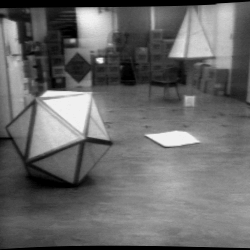
\includegraphics[width=0.6\linewidth]{img/cart_orig_left.png}
        \caption{left}
    \end{subfigure}% <- this percent sign is important 8)
    \begin{subfigure}{0.5\textwidth}
        \centering
        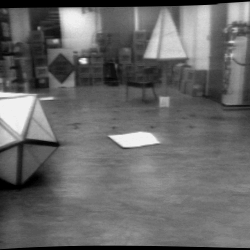
\includegraphics[width=0.6\linewidth]{img/cart_orig_right.png}
        \caption{right}
    \end{subfigure}
    \caption{An example of a stereo image.}
    \label{fig:cart_orig}
\end{figure}

An example of the type of image we used is shown in Figure~\ref{fig:cart_orig}.

\begin{figure}
    \begin{subfigure}{0.5\textwidth}
        \begin{equation*}
            \left[
            \begin{matrix}
                7 & 7 & 5 & 4 & 0 & 0 & 0 & 0 \\
                7 & 5 & 4 & 0 & 0 & 0 & 0 & 0 \\
                6 & 5 & 0 & 0 & 0 & 0 & 0 & 0 \\
                5 & 0 & 0 & 0 & 0 & 0 & 0 & 0 \\
                5 & 0 & 0 & 0 & 0 & 0 & 0 & 0 \\
                4 & 0 & 0 & 0 & 0 & 0 & 0 & 0 \\
                0 & 0 & 0 & 0 & 0 & 0 & 0 & 0 \\
                0 & 0 & 0 & 0 & 0 & 0 & 0 & 0
            \end{matrix}
            \right]
        \end{equation*}
    \caption{left}
    \end{subfigure}%
    \begin{subfigure}{0.5\textwidth}
        \begin{equation*}
            \left[
            \begin{matrix}
                7 & 6 & 5 & 3 & 0 & 0 & 0 & 0 \\
                7 & 4 & 4 & 0 & 0 & 0 & 0 & 0 \\
                6 & 4 & 0 & 0 & 0 & 0 & 0 & 0 \\
                5 & 0 & 0 & 0 & 0 & 0 & 0 & 0 \\
                5 & 0 & 0 & 0 & 0 & 0 & 0 & 0 \\
                4 & 0 & 0 & 0 & 0 & 0 & 0 & 0 \\
                4 & 0 & 0 & 0 & 0 & 0 & 0 & 0 \\
                0 & 0 & 0 & 0 & 0 & 0 & 0 & 0
            \end{matrix}
            \right]
        \end{equation*}
    \caption{right}
    \end{subfigure}
    \caption{Greedy independent 64 bit allocation for the stereo images of figure \ref{fig:cart_orig} }
    \label{fig:cart_bit_alloc}
\end{figure}

An important question in transform coding is that of bit allocation. We wish to know how many bits, i.e. how many code vectors, to assign to each DCT coefficient to optimally recover the source. The case involving a single transmitter and receiver was studied in \ref{julien}. A simple greedy algorithm optimally allocates bits to the DCT coefficients. The algorithm assumes that the $(0,0)$ coefficient (the DC coefficient) is Gaussian, while the other 63 coefficients are Laplacian \ref{julien}. An example of how this algorithm allocates bits to the images of figure \ref{fig:cart_orig} is given in figure \ref{fig:cart_bit_alloc}.

\begin{figure}
    \begin{equation*}
        \left[
        \begin{matrix}
        0.443 & -0.01  & -0.093 & -0.011 & -0.061 &   0.003 & -0.017 &  0.062 \\
        0.416 &  0.006 & -0.011 &  0.014 & -0.031 &  -0.039 &  0.003 & -0.045 \\
        0.498 & -0.061 & -0.01  &  0.074 & -0.034 &  -0.017 &  0.008 &  0.054 \\
        0.438 &  0.027 & -0.008 &  0.074 & -0.016 &   0.022 &  0.006 & -0.004 \\
        0.449 &  0.075 & -0.019 &  0.017 &  0.014 &   0.063 & -0.029 &  0.007 \\
        0.632 &  0.028 & -0.034 & -0.018 &  0.033 &  -0.037 &  0.032 &  0.061 \\
        0.765 &  0.177 & -0.032 & -0.063 & -0.033 &   0.076 & -0.001 &  0.089 \\
        0.679 &  0.148 &  0.028 &  0.04  &  0.046 &  -0.013 &  0.046 &  0.034
        \end{matrix}
        \right]
    \end{equation*}
    \caption{DCT coefficient correlation matrix of the stereo images in figure \ref{fig:cart_orig}.}
\end{figure}

\begin{figure}
    \begin{equation*}
        \left[
        \begin{matrix}
        0.654 & 0.134 & 0.054 & 0.087 & 0.077 & 0.124 & 0.119 & 0.144 \\
        0.371 & 0.072 & 0.043 & 0.059 & 0.05  & 0.063 & 0.053 & 0.048 \\
        0.273 & 0.067 & 0.065 & 0.06  & 0.055 & 0.05  & 0.062 & 0.059 \\
        0.23  & 0.056 & 0.064 & 0.053 & 0.046 & 0.045 & 0.047 & 0.039 \\
        0.242 & 0.053 & 0.05  & 0.056 & 0.047 & 0.062 & 0.058 & 0.036 \\
        0.213 & 0.064 & 0.064 & 0.05  & 0.061 & 0.052 & 0.045 & 0.059 \\
        0.238 & 0.068 & 0.07  & 0.056 & 0.048 & 0.046 & 0.042 & 0.054 \\
        0.233 & 0.081 & 0.074 & 0.066 & 0.046 & 0.05  & 0.039 & 0.049
        \end{matrix}
        \right]
    \end{equation*}
    \caption{Average DCT coefficient correlation matrix of the dataset of 39 pairs of stereo images.}
\end{figure}

The DCT computations and image manipulation was coded in Python using Pillow Imaging library and numpy.

The bit allocation problem for the two source case was not studied. We have thus omitted bit allocation from our simulations, and assigned equal bits to each component when comparing systems.

% Implementation:
% Python PILLOW library & numpy

\subsection{Design Summary}
% Summary initialization scheme in summary. We also have two stages : training stage (which is performed offline) and running stage which is used during simulation.
We review below the design of our system for processing images.

\medskip
{\noindent \bf Training Phase}
\begin{enumerate}
    \item Choose pairs of stereo images to act as the training sets;
    \item Convert pixel data of stereo images to 64 scalar pair sets of 2-D DCT coefficients;
    \item Uniformly quantize sets;
    \item Perform `Initialization Stage' quantization with splitting on each set;
    \item Perform `Channel-Optimization Stage' quantization until convergence on each set;
    \item Perform simulated annealing to find approximately optimal channel codeword mappings $b_X, b_Y$ on each set;
    \item Return to step \ref{channel_opt_stage} until satisfactory distortion is achieved.
\end{enumerate}
\medskip
{\noindent \bf Simulation Phase}
\begin{enumerate}
    \item Choose a pair of stereo images to act as the simulation set;
    \item Convert pixel data of stereo images to 64 scalar pair sets of 2-D DCT coefficients;
    \item Uniformly quantize sets;
    \item Using codebooks and channel codeword maps from training phase, find the nearest neighbour for each quantized level;
    \item Send encoded channel indices over a simulated channel;
    \item Receive indices and decode according to the centroid condition.
\end{enumerate}

% Summarize design and talk about complexity.
% [unif Q_X] -> [enc X] -> [b_X] \
%                                 --> [MAC]-- [Joint decode]
% [unif Q_Y] -> [enc Y] -> [b_Y] /

\section{Appendix: A}
Define
$q_X(x):\mathbb{R} \rightarrow \{\bar x_1,\ldots,\bar x_{L_X}\}$
and
$q_Y(y):\mathbb{R} \rightarrow \{\bar y_1,\ldots,\bar y_{L_Y}\}$
to be $L_X$- and $L_Y$-level uniform quantizers for the sources $X$ and $Y$ respectively, where the $\bar x_i-\bar x_{i-1}$ is constant for all $i\in \{2,\ldots,L_X\}$, and $\bar y_i-\bar y_{i-1}$ constant for all $i\in \{2,\ldots,L_Y\}$. Call these constants respectively $\Delta_X, \Delta_Y$.
\begin{align}
    q_X(x) = \bar x_i \in \{\bar x_1,\ldots,\bar x_{L_X}\} &\iff x \in  \left[\bar x_{i}-\frac{\Delta_X}{2},\ \bar x_i+\frac{\Delta_X}{2}\right)\\
    q_Y(y) = \bar y_i \in \{\bar y_1,\ldots,\bar y_{L_Y}\} &\iff y \in  \left[\bar y_{i}-\frac{\Delta_Y}{2},\ \bar y_i+\frac{\Delta_Y}{2}\right)
\end{align}
with the convention that $\bar x_{0}=\bar y_{0}=-\infty$, and $\bar x_{L_X+1}=\bar y_{L_Y+1}=+\infty$.

We begin our approximation by defining the uniformly quantized random variables $\bar X, \bar Y$ as follows:
\begin{align}
    \bar X = q_X(X)\\
    \bar Y = q_Y(Y)
\end{align}

With these uniformly quantized random variables in hand, we can now approximate the conditional densities $f_{Y|X}, f_{X|Y}$ by approximating the conditional pmfs of the $\bar X, \bar Y$ pair with the empirical distributions of a uniformly quantized training set $\mathcal{\bar T}$. Define $\mathcal{\bar T}$ to be the finite training set drawn from the joint pmf of the uniformly quantized pair $\bar X, \bar Y$. Define $p_{\bar Y|\bar X}(\bar y|\bar x),p_{\bar X|\bar Y}(\bar x|\bar y)$ respectively as the conditional \emph{empirical} pmfs of $\bar Y$ given $\bar X$ and $\bar X$ given $\bar Y$ according to the training set $\mathcal{\bar T}$. Our approximation is thus in two stages, namely the uniform quantization step, and the training set estimation step. Each of these contributes in a different way to the approximation error. We have:
\begin{align}
    p_{\bar Y|\bar X}(q_Y(y)|q_X(x)) \approx 
        P(\bar Y=q_Y(y) | \bar X=q_X(x)) \approx
            f_{Y|X}(y|x)\\
    p_{\bar X|\bar Y}(q_X(x)|q_Y(y)) \approx 
        P(\bar X=q_X(x) | \bar Y=q_Y(y)) \approx
            f_{X|Y}(x|y)
\end{align}

Writing out $p_{\bar Y|\bar X}, p_{\bar X|\bar Y}$ in terms of our uniformly quantized training set $\mathcal{\bar T}$ gives:
\begin{align}
    p_{\bar Y|\bar X}(\bar y_n | \bar x_m)=\frac{
            \left|\{(\bar x,\bar y)\in \mathcal{\bar T}\ |\ \bar x = \bar x_m, \bar y = \bar y_n\}\right|
        }{
            \left|\{(\bar x,\bar y)\in \mathcal{\bar T}\ |\ \bar x = \bar x_m\}\right|
        },\quad (\bar x_n, \bar y_m)\in \{x_1,\ldots,x_{L_X}\}\times\{y_1,\ldots,y_{L_Y}\}\\
    p_{\bar X|\bar Y}(\bar x_m | \bar y_n)=\frac{
            \left|\{(\bar x,\bar y)\in \mathcal{\bar T}\ |\ \bar x = \bar x_m, \bar y = \bar y_n\}\right|
        }{
            \left|\{(\bar x,\bar y)\in \mathcal{\bar T}\ |\ \bar y = \bar y_n\}\right|
        },\quad (\bar x_n, \bar y_m)\in \{x_1,\ldots,x_{L_X}\}\times\{y_1,\ldots,y_{L_Y}\}
\end{align}

We now rewrite our approximated versions of equations \eqref{eq:problem_1}, \eqref{eq:problem_2}, \eqref{eq:problem_3} (and their counterparts in $Y$). Define $T_{\bar X}(q_X(x)),T_{\bar Y}(q_Y(y)),M_{\bar X}(q_X(x),j),M_{\bar Y}(q_Y(y),i),S_{\bar X}(q_X(x),j),S_{\bar Y}(q_Y(y),i)$ as these approximations:
\begin{align*}
    T_{\bar X}(q_X(x)) &= \sum_{n=1}^{L_Y}(\bar y_n)^2p_{\bar Y|\bar X}(\bar y_n|q_X(x)) \approx E[Y^2 | X = x]\\
    T_{\bar Y}(q_Y(y)) &= \sum_{m=1}^{L_X}(\bar x_m)^2p_{\bar X|\bar Y}(\bar x_m|q_Y(y)) \approx E[X^2 | Y = y]\\
    M_{\bar X}(q_X(x),j) &= 
        \frac{
            |\mathcal{\bar T}|
        }{
            |\{(\bar x, \bar y)\in \mathcal{\bar T}\ |\ \bar y\in R_j^{\bar Y}\}|
        } \sum_{\bar y_n\in R_j^{\bar Y}}\bar y_np_{\bar Y|\bar X}(\bar y_n|q_X(x))
        \approx E[Y|X=x,Y\in R_j^{Y}]\\
    M_{\bar Y}(q_Y(y),i) &= 
        \frac{
            |\mathcal{\bar T}|
        }{
            |\{(\bar x,\bar y)\in \mathcal{\bar T}\ |\ \bar x\in R_i^{\bar X}\}|
        } \sum_{\bar x_m\in R_i^{\bar X}}\bar xp_{\bar X|\bar Y}(\bar x_m|q_Y(y))
        \approx E[X|Y=y,X\in R_i^{X}]\\
    S_{\bar X}(q_X(x),j) &= 
        \sum_{\bar y_n\in \{\bar y_1,\ldots,\bar y_{L_Y}\}\cap R_j^{\bar Y}}p_{\bar Y|\bar X}(\bar y_n|q_X(x)) 
        \approx P(Y\in R_j^{Y}|X=x)\\
    S_{\bar Y}(q_Y(y),i) &= 
        \sum_{\bar x_m\in \{\bar x_1,\ldots,\bar x_{L_X}\}\cap R_i^{\bar X}}p_{\bar X|\bar Y}(\bar x_m|q_Y(y)) 
        \approx P(X\in R_i^{X}|Y=y)
\end{align*}
Note that we used the notation $R_i^{\bar X}, R_j^{\bar Y}$ to indicate that these are the encoding partitions for the uniformly quantized random variables $\bar X$ and $\bar Y$ respectively.

\section{Appendix B}
Let $M_{(i,j)}$ be given by:
\begin{align}
    M_{(i,j)} &=
    \sum_{(\bar x_m,\bar y_n)\in R_i^{\bar X}\times R_j^{\bar Y}}p(\bar x_m,\bar y_n)
\end{align}
and let $S_{(i,j)}^{\bar X}$, $S_{(i,j)}^{\bar Y}$ be given by:
\begin{align}
    S^{\bar X}_{(i,j)} &=
    \sum_{(\bar x_m,\bar y_n)\in R_i^{\bar X}\times R_j^{\bar Y}}\bar x_m p(\bar x_m,\bar y_n)\\
    S^{\bar Y}_{(i,j)} &=
    \sum_{(\bar x_m,\bar y_n)\in R_i^{\bar X}\times R_j^{\bar Y}}\bar y_n p(\bar x_m,\bar y_n)
\end{align}
where $p(\bar x_m,\bar y_n)$ is the joint empirical distribution of $\bar X,\bar Y$ according to $\mathcal{\bar T}$:
\begin{align}
    p(\bar x_m,\bar y_n)=\frac{1}{|\mathcal{\bar T}|}\left|\{(\bar x,\bar y)\in\mathcal{\bar T}\ |\ (\bar x,\bar y)=(\bar x_m,\bar y_n)\}\right|
\end{align}

\section{Appendix C}

We now describe the algorithm in terms of our functions. We require a few parameters that together control the amount of time spent searching the state space. Define:
\begin{equation}
    \{T_i=10,T_f=0.00025,R=0.8,\phi_{max}=5,\psi_{max}=200\}
\end{equation}
In words, these are respectively: the initial `temperature', the final `temperature', the `cooling rate', the number of energy drops until we lower the temperature, the number rejected new states until we lower the temperature. These values are taken from \ref{}. We stop our search when our timing variable the `temperature' equals $T_f$.

\begin{enumerate}
    \item Initialize $b_X, b_Y$ to the identity maps:
    \begin{align}
        b_X(i) = i,  \quad\forall i\in \{1,\ldots,N_X\}\\
        b_Y(j) = j, \quad\forall j\in \{1,\ldots,N_Y\}
    \end{align}
    \item Initialize temperature $T$; let $T=T_i$.
    \item Initialize counters; let $\phi=0$, $\psi=0$
    \item Initialize `best' channel index maps; let
    \begin{align}
        b_{X_{best}}&=b_X\\
        b_{Y_{best}}&=b_Y
    \end{align}
    \item \label{anneal_loop}
    At random, choose $i_1, i_2\in \{1,\ldots,N_X\}$, choose $j_1,j_2\in \{1,\ldots,N_Y\}$. Define $b'_X,b'_Y$ as follows:
    \begin{align}
        b'_X(i) = 
            \begin{cases}
                b_X(i_1) &\mbox{if } i=i_2\\
                b_X(i_2) &\mbox{if } i=i_1\\
                b_X(i)  &\mbox{otherwise}
            \end{cases}\\
        b'_Y(i) = 
            \begin{cases}
                b_Y(j_1) &\mbox{if } j=j_2\\
                b_Y(j_2) &\mbox{if } j=j_1\\
                b_Y(j)  &\mbox{otherwise}
            \end{cases}
    \end{align}
    \begin{enumerate}
        \item If $D_C(b'_X,b'_Y)<D_C(b_X,b_Y)$, accept the change; let
            \begin{align}
                b_X&=b'_X\\
                b_Y&=b'_Y
            \end{align}
        \item If $D_C(b'_X,b'_Y)\ge D_C(b_X,b_Y)$, accept the change with probability $\exp(\frac{-(D_C(b'_X,b'_Y)- D_C(b_X,b_Y))}{T})$.
        \item Otherwise, keep the current state.
    \end{enumerate}
    \item If $D_C(b_X, b_Y) < D_C(b_{X_{best}}, b_{Y_{best}})$, store this `best' state; let
    \begin{align}
        b_{X_{best}}&=b_X\\
        b_{Y_{best}}&=b_Y
    \end{align}
    \item
    \begin{enumerate}
        \item If we accepted the change, increment $\phi$; let $\phi=\phi+1$
        \item Otherwise, increment $\psi$; let $\psi=\psi+1$
    \end{enumerate}
    \item
    \begin{enumerate}
        \item If $\psi=\psi_{max}$, reset $\psi$, lower temperature; let
        \begin{align}
            \psi &= 0\\
            T &= R\cdot T
        \end{align}
        \item Otherwise, if $\phi=\phi_{max}$, reset $\phi$, lower temperature; let
        \begin{align}
            \phi &= 0\\
            T &= R\cdot T
        \end{align}
        \item Otherwise, leave temperature unchanged.
    \end{enumerate}
    \item 
    \begin{enumerate}
        \item If $T > T_f$, go back to step \ref{anneal_loop}
        \item Otherwise, restore best state; let
        \begin{align}
            b_X&=b_{X_{best}}\\
            b_Y&=b_{Y_{best}}
        \end{align}
    \end{enumerate}
\end{enumerate}
